% !TeX TXS-program:compile = txs:///pdflatex/[--shell-escape]

\documentclass[9pt]{beamer}
\usetheme{Madrid}
\usecolortheme{beaver}
\usepackage{amsmath,amssymb,amsthm,asymptote,graphicx}
\usepackage{graphics}
% \usepackage{bisvslides}
\usepackage{arcs}
\usepackage{tikz}
\graphicspath{{./images}}

\newcounter{problem}[section]

\newenvironment{probslide}[3][]{%
    \refstepcounter{problem}\begin{frame}[t]%
	{Problem \thesection.\theproblem 
        \def\temp{#2}\ifx\temp\empty
            %
        \else
            \ - \temp%
        \fi}
    {#3}}%
	{\end{frame}}

% \newenvironment{Example}[2][Example]
%     {This is an #1. You gave #2 as an argument. The rest will be bold: \bfseries}
%     {}
% \textbf{Problem~\theproblem. #1
% \newenvironment{bsmi}{\begin{CJK}{UTF8}{bsmi}}{\end{CJK}}

\title{Advanced Topics}
\subtitle{Mathcounts 22 - Session 5}
\author{Rohan D., Derrick L., Shivani V.}
\institute{BISV Mathcounts Club 22}
\date{January 31, 2023}

%\maketitle
%~~~~~~~~~~~~~~~~~~~~~~~~~~~~~~~~~~~~~~~~~~~~~~~~~~~~~~~~~~~~~~~~~~~~~~~~~~~~~~
% Informations
%\title{TEMPLATE}

%\titlegraphic{assets/gkg.png} %change this to your preferred logo or image(the image is located on the top right corner).
%~~~~~~~~~~~~~~~~~~~~~~~~~~~~~~~~~~~~~~~~~~~~~~~~~~~~~~~~~~~~~~~~~~~~~~~~~~~~~~

\begin{document}

% Generate title page
\begin{frame}
    \titlepage        
\end{frame}
% \setbeamertemplate{footline}[miniframes Madrid]

\setcounter{section}{2}
\section{Intermediate Practice Problems}
% Used again in 2022 Session 5
\refstepcounter{problem}
\begin{frame}[t, fragile]{Problem \thesection.\theproblem}
    \begin{block}{}[MATHCOUNTS]
    % Concept: Geometry • Difficulty: 4 • Answer: 50 • Solution Available: Yes (Hide) • Report an error with this problem.

 Right $\triangle ABC$ with legs $AB=3$ cm and $CB=4$ cm is rotated about one of its legs. What is the greatest possible number of cubic centimeters in the volume of the resulting solid? Express your answer to the nearest whole number.
	
	
    \end{block}
\end{frame}

% Difficulty: 5
\refstepcounter{problem}
\begin{frame}[t, fragile]{Problem \thesection.\theproblem}
    \begin{block}{}[MATHCOUNTS Handbook 2022-2023, \#246]
    A standard six-sided die is rolled twice. What is the expected value of the sum of the squares of the two numbers rolled? Express your answer as a decimal to the nearest tenth.
    
	
    \end{block}
\end{frame}


\refstepcounter{problem}
\begin{frame}[t, fragile]{Problem \thesection.\theproblem}
    \begin{block}{}[MATHCOUNTS Chapter 2022, Team \#8]
    In a regular icosagon (20-sided polygon), all the diagonals are drawn. If a diagonal is selected at random, what is the probability of selecting a diagonal that is neither the shortest possible length nor the longest possible length? Express your answer as a common fraction.
    
	
    \end{block}
\end{frame}

% Difficulty: 6
\refstepcounter{problem}
\begin{frame}[t, fragile]{Problem \thesection.\theproblem}
    \begin{block}{}[MATHCOUNTS Handbook 2022-2023, \#236]
    An octahedron is in the interior of a cube, and each of its vertices is the center of a face of the cube. What is the ratio of the surface area of the inner octahedron to the surface area of the outer cube? Express your answer as a common fraction in simplest radical form.
    \end{block}
    \begin{center}
        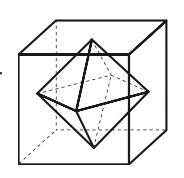
\includegraphics[]{hb_22_236}
    \end{center}

\end{frame}

% Difficulty: 7
\refstepcounter{problem}
\begin{frame}[t, fragile]{Problem \thesection.\theproblem}
    \begin{block}{}[MATHCOUNTS Handbook 2022-2023, \#239]
    Twenty-five cards are marked with the numbers 1 through 25. Amira randomly picks two cards without replacement. Blanca then randomly picks two of the remaining cards without replacement. What is the probability that at least one of Blanca’s cards has a number greater than at least one of Amira’s cards?
Express your answer as a common fraction.
    
	
    \end{block}
\end{frame}

% Difficulty: 7
\refstepcounter{problem}
\begin{frame}[t, fragile]{Problem \thesection.\theproblem}
    \begin{block}{}[MATHCOUNTS Handbook 2022-2023, \#250]
The figure shows 23 white unit cubes and 4 gray cubes randomly arranged and assembled into a large 3 × 3 × 3 cube. The number of gray squares appearing on the surface of the cube is then counted. One such arrangement, shown here, has 10 gray squares on its surface. What is the expected value of the number of gray squares that will appear on the surface of the cube?
    \end{block}
    \begin{center}
        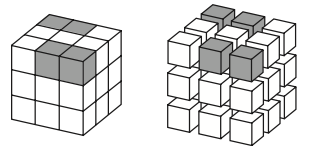
\includegraphics[]{hb_22_250}
    \end{center}    
\end{frame}

% Used again in 2022
\refstepcounter{problem}
\begin{frame}[t, fragile]{Problem \thesection.\theproblem}
    \begin{block}{}[2017 AMC 10B, \#13]
There are $20$ students participating in an after-school program offering classes in yoga, bridge, and painting. Each student must take at least one of these three classes, but may take two or all three. There are $10$ students taking yoga, $13$ taking bridge, and $9$ taking painting. There are $9$ students taking at least two classes. How many students are taking all three classes?
    
	
    \end{block}
\end{frame}

% Used again in 2022 Session 5
\refstepcounter{problem}
\begin{frame}[t, fragile]{Problem \thesection.\theproblem}
    \begin{block}{}[MATHCOUNTS Handbook 21-22, \#237]
    % Difficulty: 6, may use calculator
    The numbers 1 through 10 are marked with points on the number line as shown. Two distinct points are chosen at random from these points. What is the expected value of the distance between the two points? Express your answer as a decimal to the nearest tenth.  \textit{May use calculator.}
	
    \end{block}
    \begin{center}

        \begin{asy}
            unitsize (0.7cm);
            
            draw ((0, 0)--(11,0), black+1.25, Arrows(4));
            for (int i = 1; i < 11; ++i) {
                dot ((string)i, (i, 0), S);
            }
        \end{asy}
        \end{center}
        
    
\end{frame}

\refstepcounter{problem}
\begin{frame}[t, fragile]{Problem \thesection.\theproblem}
    \begin{block}{}[MATHCOUNTS Handbook 21-22, \#211]
    The net of a certain rectangular pyramid is composed of a 6-inch by 12-inch rectangle surrounded by two pairs of congruent isosceles triangles as shown. Each triangle has two sides of length 7 inches. What is the volume of the pyramid?


	
	
    \end{block}
    \begin{center}
        \begin{asy}
            unitsize (0.25cm);
            import olympiad;
    
            pair O, A, B, C, D, E, F, G, H;
            real x, y;
    
            O = (0, 0);
            A = (-6, -3);
            B = (6, -3);
            C = (6, 3);
            D = (-6, 3);
    
            x = sqrt(7**2-3**2);
            E = (-6-x, 0);
            G = rotate (180, O) * E;
            
            F = extension (E, A, O, (0, -1));
    
            H = rotate (180, O) * F;
    
            draw (A--B, L="12 in", dashed);
            draw (B--C--D, dashed);
            draw (D--A, L="6 in", dashed);
    
            draw (E--A, L="7 in");
            draw (A--F, L="7 in");
    
            draw (F--G--H--E);
    
    
            add(pathticks(E--A,1,0.5,0,25));
            add(pathticks(A--F,1,0.5,0,25));
            add(pathticks(F--B,1,0.5,0,25));
            add(pathticks(B--G,1,0.5,0,25));
            add(pathticks(G--C,1,0.5,0,25));
            add(pathticks(C--H,1,0.5,0,25));
            add(pathticks(H--D,1,0.5,0,25));
            add(pathticks(D--E,1,0.5,0,25));
    
            draw (rightanglemark (B, A, D, 15));
            draw (rightanglemark (C, B, A, 15));
            draw (rightanglemark (D, C, B, 15));
            draw (rightanglemark (A, D, C, 15));
    
    
        \end{asy}
    \end{center}
    
\end{frame}

% Used again in 2022 Session 5
\refstepcounter{problem}
\begin{frame}[t, fragile]{Problem \thesection.\theproblem}
    \begin{block}{}[MATHCOUNTS 2015 State Target \#6]
The shape below can be folded along the dashed lines and taped together along
the edges to form a three-dimensional polyhedron. All lengths in the diagram are
given in inches. What is the volume of the resulting polyhedron? Express your
answer in simplest radical form.

    
	
    \end{block}
    \begin{center}
        \begin{asy}
            import olympiad;
            unitsize (0.35cm);
    
            pair A, B, C, D, E, F, G, H, I, J;
    
            A = (0, 0);
            B = (4, 0);
            C = (4, 7);
            D = (0, 7);
            E = (-4, 0);
            F = (-4, 4);
            G = (8, 0);
            H = (8, 4);
            I = rotate (-60, A) * B;
            J = (2, 7 + sqrt(21));
    
            draw (A--B, L="4", dashed);
            draw (D--A, L="7", dashed);
            draw (B--C, L="7", dashed);
            draw (C--D, L="4", dashed);
            draw (A--I, L="4");
            draw (I--B, L="4");
            draw (B--G, L="4");
            draw (G--H, L="4");
            draw (H--C, L="5");
            draw (C--J, L="5");
            draw (E--A, L="4");
            draw (F--E, L="4");
            draw (D--F, L="5");
            draw (J--D, L="5");
            draw (rightanglemark (D, A, E, 10));
            draw (rightanglemark (A, E, F, 10));
            draw (rightanglemark (G, B, C, 10));
            draw (rightanglemark (H, G, B, 10));
        \end{asy}
    \end{center}
    
\end{frame}

% Used again in 2022
% Mass Point
\refstepcounter{problem}
\begin{frame}[t, fragile]{Problem \thesection.\theproblem}
    \begin{block}{}[MATHCOUNTS 2015 State Sprint \#28]
In regular pentagon $ABCDE,$ point $M$ is the midpoint of side $AE,$ and segments
$AC$ and $BM$ intersect at point $Z.$ If $ZA = 3,$ what is the value of $AB?$ Express
your answer in simplest radical form.

	
    \end{block}
\end{frame}

% Geometric Probability
\refstepcounter{problem}
\begin{frame}[t, fragile]{Problem \thesection.\theproblem}
    \begin{block}{}[MATHCOUNTS National 2018, Target \#6]
    Micaela randomly chooses a real number $ w $ between -20 and 20. What is the probability that the graphs of $ x -|y| = w $ and $ x^2 + y^2 = 50 $ intersect at exactly two points? Express your answer as a decimal to the nearest hundredth.
    
	
    \end{block}
\end{frame}

% Used again in 2022 Session 5
\refstepcounter{problem}
\begin{frame}[t, fragile]{Problem \thesection.\theproblem}
    \begin{block}{}[MATHCOUNTS Handbook 21-22, \#213]
    A circle is drawn inside triangle $ABC$ so that it is tangent to all three sides of the triangle. Triangle $ABC$ has perimeter $24$ cm and area $8 \text{ cm}^2$. What is the radius of the circle? Express your answer as a common fraction.
	
	
    \end{block}
\end{frame}

% Used again in 2022 Session 5
\refstepcounter{problem}
\begin{frame}[t, fragile]{Problem \thesection.\theproblem}
    \begin{block}{}[MATHCOUNTS Handbook 21-22, \#220]
    There are 30 balls, each a different color, and 30 boxes in the same 30 colors. One ball is placed in each box. How many ways can the balls be placed so that exactly 3 of the balls do not match the color of the box they are in?
	
	
    \end{block}
\end{frame}

% Used again in 2022 Session 5
\refstepcounter{problem}
\begin{frame}[t, fragile]{Problem \thesection.\theproblem}
    \begin{block}{}[MATHCOUNTS Handbook 21-22, \#224]
    Danny and Mila are playing tic-tac-toe. Their game board is shown. A fly lands randomly on one of the squares of their game board and then randomly moves to one of the squares that is vertically or horizontally adjacent to the square it landed on. What is the probability that the fly ends on a square marked with an X? Express your answer as a common fraction.
	
    \end{block}
    \begin{center}
        \begin{asy}
            unitsize (0.75cm);
    
            for (int i = 0;  i < 4; ++i) {
                draw ((i, 0) -- (i, 3));
                draw ((0, i) -- (3, i));
            }
            label ("O", (1.5, 1.5));
            label ("O", (0.5, 2.5));
            label ("X", (1.5, 2.5));
            label ("X", (2.5, 2.5));
        \end{asy}
        \end{center}
        
    
\end{frame}
%--------------
% Used again in 2022 Session 5
\refstepcounter{problem}
\begin{frame}[t, fragile]{Problem \thesection.\theproblem}
    \begin{block}{}[MATHCOUNTS 2018 National, Sprint \#23]
    Xena and Yolanda toss an unfair coin that lands heads up $ 75\% $ of the time. If the coin lands heads up, Xena gets a point. Otherwise, Yolanda gets a point. The game ends when one player has a two-point lead over the other, and the player with the two-point lead is the winner. What is the probability that Xena wins the game? Express your answer as a common fraction.
    
	
    \end{block}
\end{frame}
%--------------

% Used again in 2022 Session 5
\refstepcounter{problem}
\begin{frame}[t, fragile]{Problem \thesection.\theproblem}
    \begin{block}{}[MATHCOUNTS 2018 National, Sprint \#24]
    The figure shows isosceles right triangle $ ABC $ with $ AC=BC=16 $ units. Triangle $ ABD $ is constructed within triangle $ ABC $ with vertex $ D $ on side $ AC $ and $ AD = 4 $ units. Point $ E $ is drawn on side $ AB $ to form isosceles right triangle $ ADE $. A series of isosceles right triangles is constructed within triangle $ ABD $, such that the hypotenuse of each lies on side $ AB $, the 90-degree vertex of each lies on segment $ BD $, and each shares a vertex with the preceding triangle in the series, as shown. What is the combined area of the series of isosceles right triangles within triangle $ ABD $? Express your answer as a common fraction.    

	
    \end{block}
    \begin{center}
        \begin{asy}
            import olympiad;

            unitsize(0.35cm);
            pair A, B, C, D, E, F, G, H, I, J, K, L;

            A = (0,0);
            B = (16, 0);
            C = (8, 8);
            D = (2, 2);
            E = (4, 0);

            F = (E.x+(3/4)*2, (3/4)*2);
            G = (E.x+(3/4)*4, 0);

            H = (G.x+(3/4)*(3/4)*2, (3/4)*(3/4)*2);
            I = (G.x+(3/4)*(3/4)*4, 0);

            J = (I.x+(3/4)*(3/4)*(3/4)*2, (3/4)*(3/4)*(3/4)*2);
            K = (I.x+(3/4)*(3/4)*(3/4)*4, 0);

            L = (K.x+(3/4)*(3/4)*(3/4)*(3/4)*2, (3/4)*(3/4)*(3/4)*(3/4)*2);

            draw(A--B--C--cycle);
            draw(B--D--E--F--G--H--I--J--K--L);

            draw(rightanglemark(A, C, B));
            draw(rightanglemark(A, D, E));
            draw(rightanglemark(E, F, G));
            draw(rightanglemark(G, H, I));
            draw(rightanglemark(I, J, K));

            label("$A$", A, SW);
            label("$B$", B, SE);
            label("$C$", C, N);
            label("$D$", D, NW);
            label("$E$", E, S);
            label("$F$", F, N);
            label("$G$", G, S);
            label("$16$", B--C, NE);
            label("$4$", A--D, NW);

            label("$\ldots$", (L.x+0.4, L.y/2));
        \end{asy}
    \end{center}
    

\end{frame}

\section{Challenge Problems}
\refstepcounter{problem}
\begin{frame}[t, fragile]{Problem \thesection.\theproblem}
    \begin{block}{}[2001 AIME I, \#7]
    Triangle $ABC$ has $AB=21$, $AC=22$ and $BC=20$. Points $D$ and $E$ are located on $\overline{AB}$ and $\overline{AC}$, respectively, such that $\overline{DE}$ is parallel to $\overline{BC}$ and contains the center of the inscribed circle of triangle $ABC$. Then $DE=m/n$, where $m$ and $n$ are relatively prime positive integers. Find $m+n$.	

    \textit{Hint: The incenter is at the intersection of angle bisectors.}

	
    \end{block}
\end{frame}

\refstepcounter{problem}
\begin{frame}[t, fragile]{Problem \thesection.\theproblem}
    \begin{block}{}[1998 AIME, \# 9]
    Two mathematicians take a morning coffee break each day. They arrive at the cafeteria independently, at random times between 9 a.m. and 10 a.m., and stay for exactly $m$ minutes. The probability that either one arrives while the other is in the cafeteria is $40 \%,$ and $m = a - b\sqrt {c},$ where $a, b,$ and $c$ are positive integers, and $c$ is not divisible by the square of any prime. Find $a + b + c.$
	
	
    \end{block}
\end{frame}

\refstepcounter{problem}
\begin{frame}[t, fragile]{Problem \thesection.\theproblem}
    \begin{block}{}[HMMT 2003]
    Find the smallest $n$ such that $n!$ ends in 290 zeroes.
	
	
    \end{block}
\end{frame}

\end{document}